\chapter{Evaluation and Discussion}
The first recreation of the malicious document and payload led us to a conclusion that we alluded to previously -- the
mechanism used to drop the payload and execute it \emph{no longer works as described in the original article by Hossein
Jazi}. 

The primary test environment we used to evaluate the effectiveness was a system running the Windows 10 operating system.
We decided to use this operating system as the basis for our testing as it's freely available for use in virtual
machines from Microsoft websites and is one of the more widely used operating systems as of the time of writing and the
time of the attack. Windows 11 began rolling out to users around in late 2021, putting it a few months behind the
attack, which was observed in April 2021 \cite{jazi-article, win11-rollout}. 

Some factors that could challenge or dispute our conclusions are the fact that we didn't have access to the original
payload files, meaning we had to guess to some parts of the implementation. The first part we had to recreate was the
image conversion mechanism, which we obtained from a document analysis dump after some searching. The second part that
we couldn't accurately recreate due to a lack of information was the payload concealment within the image file, which
wasn't dissected in the original article. 

\section{Issues with Malware Execution}
It is important to note that we tried to stick as closely as possible to the original malware, changing only minor
things. We made some changes to make debugging easier, such as not using the original payload locations
(\verb+C:\Users\<user>\AppData\Local\Temp+ and \verb+C:\Users\Public\Libraries+) and instead using local folders in a
test directory.

When recreating the parts of the malware that were not covered, we tried to hold ourselves as closely as possible to
indicators described within the original article. For example, the \verb+Decode+ function used to decode strings in
the macro was not provided, but it was mentioned that the strings were Base 64 encoded, so we wrote our own Base 64
decoding algorithm.

\subsection{Issues in the Macro}
The issues with the recreation started in the very first part of the execution chain. Aside from the aforementioned
lacking functions which we had to write ourselves or find elsewhere, there were some issues stemming from the
construction of the document itself. For example, the original payload contained multiple images, with only one of them
being malicious, meaning we had to change the file name reference in the macro to point to the correct image in our
document.

The next issues arose in a subroutine called \verb+Show+ which was responsible for protecting the document. There were
three function calls that failed and caused the macro to crash, all relating to the reconstruction of the document,
addressing elements that were not present in our recreated document. Interestingly, the original document seems to have
been protected with a password, or else the \verb+Application.ActiveDocument.Unprotect+ function would fail, crashing
the macro.

\begin{lstlisting}[language=VBScript, caption={Failing function calls from the document protection subroutine}][H]
    Application.ActiveDocument.Unprotect Password:="taifehjRTYB\$%^45"
    Application.ActiveDocument.Shapes(1).Visible = False
    Bookmarks("main").Range.Font.Hidden = False
\end{lstlisting}

%TODO: Check this part to make sure!
A surprising issue that came up in the implementation was also a failure in string concatenation, where for some reason,
the concatenation of \verb+Value & " " & CreatedImageBMPFilePath+ evaluated simply to \verb+Value+ whereas the
concatenation of \verb+"mshta" & " " & CreatedImageBMPFilePath+ evaluated correctly. Thus, we had to change the
concatenation to not use the de-obfuscated value variable, defeating the purpose of hiding that data in the first place,
leading to a further inefficiency in the malware.

Finally, the largest problem in the macro execution stems from the \verb+WIA_ConvertImage+ function. This function was
expected to convert the malicious \acrshort{PNG} file into \acrshort{BMP}, extracting the malicious payload in the
process. However, this was not the case. The conversion process converted the image properly, however all the other
bytes of the file were left garbled, replaced mostly with \verb+00+ and \verb+ff+ bytes, corresponding to series of
all zeroes and all ones respectively. The \verb+binwalk+ signature also doesn't match the one showed in the article,
notably not displaying that the file contains \acrshort{HTML} (as the original payload did), because it has been 
destroyed in the conversion process.

\begin{figure}[H]
  \centering
  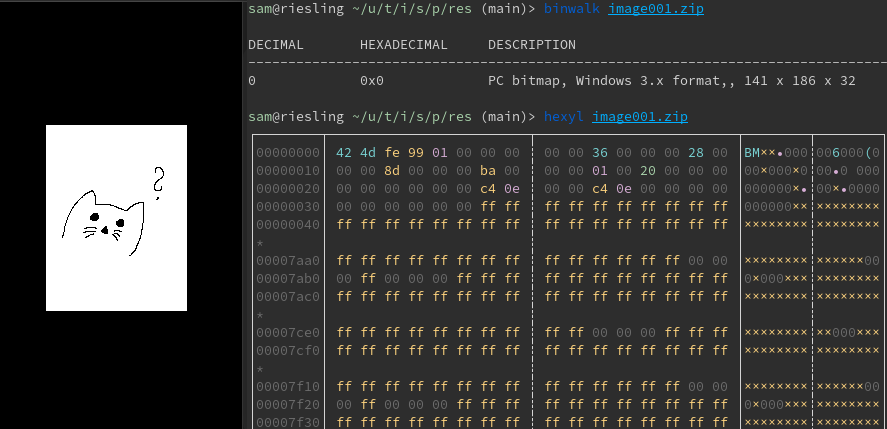
\includegraphics[width=0.9\textwidth]{figures/faulty_bmp_conversion.png}
  \label{malicious_document}
  \caption{The result of the image conversion -- with the garbled payload}
\end{figure}

We are not sure if this is due to some error in the payload creation process on our part, or if the faulty conversion
mechanism has been patched by Microsoft in the wake of the original malware attack. We have reached out to the author of
the original article for comment, but we haven't received a response yet.

In trying to find out if there was any error on our part, we tried various ways of appending the compressed payload to 
the \acrshort{PNG} as well as attaching an uncompressed payload to no avail.
We tried the following:
\begin{itemize}
    \item attaching the compressed payload as-is to the end of the \acrshort{PNG},
    \item removing the Zlib header from the compressed payload, then attaching it to the end of the \acrshort{PNG},
    \item appending the uncompressed payload to the end of the \acrshort{PNG},
    \item removing the Zlib header from the compressed payload and removing the \verb+IEND+ image trailer from the
        \acrshort{PNG} data, effectively appending our data to the \acrshort{PNG} data stream, then adding the
        \verb+IEND+ image trailer to the end of the appended data.
\end{itemize}

None of these approaches were able to successfully replicate the behaviour of the original malware. The implementation
source code we provide uses the final approach, as we deem it to be the most robust and likely to be used in the real
attack.

This fact alone makes this attack \emph{irreproducible} using the same methods as documented in the malware post-mortem.

\section{Running the Malware}
Though the image conversion mechanism didn't work as intended, if we instead placed a pre-converted image containing the
payload and let the malicious document execute using this pre-converted image as its payload, all the other parts worked
as expected. By removing the conversion and providing the \acrshort{HTA} payload to the document directly we were able
to make the malware work and reproduce its behaviour. 

\begin{figure}[H]
  \centering
  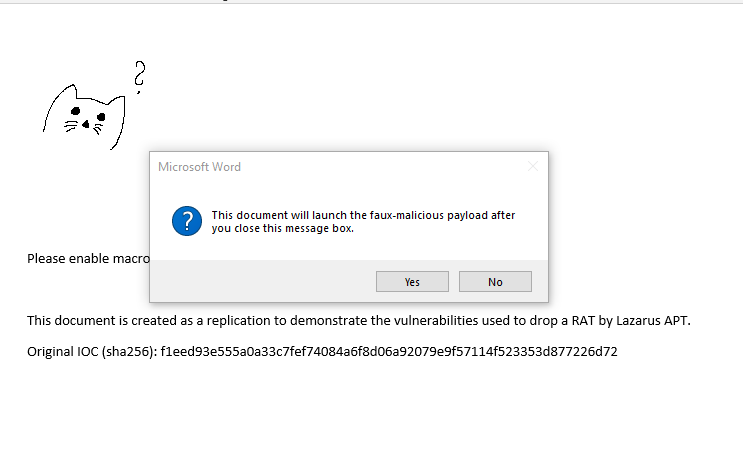
\includegraphics[width=0.9\textwidth]{figures/macro_popup.png}
  \label{malware-msgbox}
  \caption{Malware execution - the pop-up warning the user the execution was about to start}
\end{figure}

\begin{figure}[H]
  \centering
  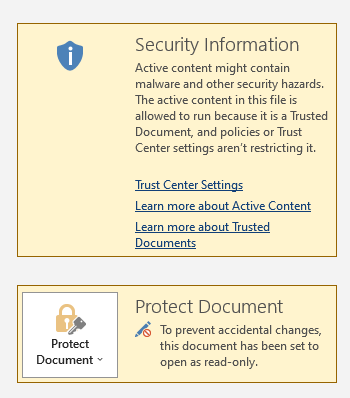
\includegraphics[scale=0.6]{figures/document_protected.png}
  \label{malware-doc-protected}
  \caption{Malware execution - the document protects itself from user changes}
\end{figure}

\begin{figure}[H]
  \centering
  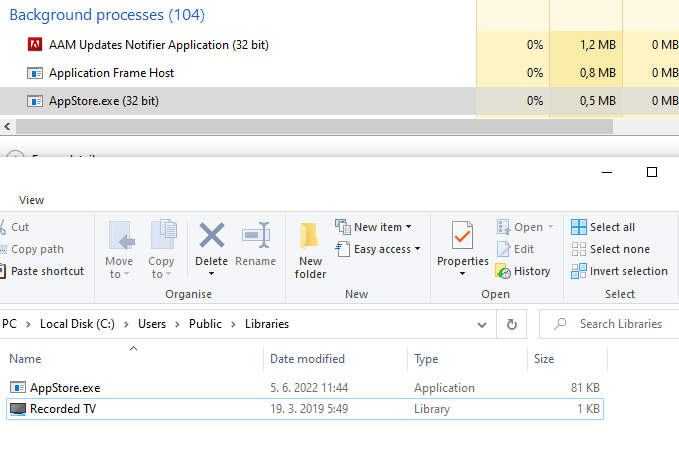
\includegraphics[width=0.9\textwidth]{figures/malware_dropped.png}
  \label{malware-payload-running}
  \caption{Malware execution - the \acrshort{HTA} payload drops the executable, 
  and it is seen running in the task manager}
\end{figure}

\section{Discussion}
After attempting to recreate the malware attack as faithfully as possible we have come to the conclusion that it cannot
be reproduced with the available resources. This comes down to one of two options, which we have already mentioned
throughout our evaluation:
\begin{enumerate}
    \item the faulty conversion mechanism exploited in \verb+WIA_ConvertImage+ has been patched,
    \item a functioning image compression methodology was not divulged, and we were unable to replicate it.
\end{enumerate}

We lean more towards the first option, as the compression mechanism used is relatively simple, and we struggle to
think of a way it could be further abused by the attackers in ways we could not find. Though we have been unable to find
any patch notes for the Microsoft Office suite that would indicate that the \acrfull{WIA} image conversion
functionality has been patched with regard to this vulnerability, that is not necessarily telling.

Reporting software vulnerabilities, whether they have been patched is a tricky subject, since it doesn't only
give information to users and systems administrators to combat the threat, but also gives information to attackers who
can use this information to attack systems vulnerable to the disclosed threat \cite{vuln-disclosure}. While there are
pros and cons to this disclosure, when it comes to closed source software such as the Microsoft Office suite it is up to
the company to decide how it handles vulnerability disclosure. 

Though research on which approach is optimal does not have an all-encompassing answer, it has been shown that disclosing 
vulnerabilities, even if they are patched at the time of disclosure, increases attack frequency in the short term 
\cite{vuln-disclosure, vuln-disclosure-impact}. It is possible that Microsoft chose not to disclose the patching of 
the vulnerability for this reason.

We tested all the parts of the attack in isolation and found all of them to work, \emph{except} the image conversion,
which was at the core of this attack. The other parts of the malware are all common operations that were not used in 
an unexpected manner in the attack. For example, using \acrshort{mshta} to execute a file within a \acrshort{VBA} macro,
while strange and potentially dangerous, isn't inherently malicious and works exactly as intended, executing the file.

While the faulty image conversion would satisfy our definition of malware, causing the program (\acrshort{WIA} in this case) 
to do what the attacker wants, regardless of run-time correctness, other parts of the malicious document do not. Hence,
we theorise that only this part of the malware execution process needed patching, and we think this has been done, due
to our inability to reproduce the malware attack in its entirety specifically due to the \acrshort{WIA} image conversion
not exhibiting the unwanted conversion behaviour.

% TODO: Test on Win7

% --------------------------------------------------
% Notes
% --------------------------------------------------
\clearpage
\begin{itemize}
    \item how did you evaluate that you reached your goals?
    \item did you use specific methods to do so? (e.g., a user study, a case study, usage scenario, 
    formal mathematical proof, performance tests, (visual) comparison to state of the art, ...)
    \item explain methods and results of this evaluation
    \item discuss the results: here you should refer back to the most closely related work. Now
    you can say why your new thing is better (given the metrics outlined in the
    motivation).
    \item discuss lessons learned and unexpected finding
\end{itemize}
\clearpage
